%==================================================================================================
%   LUKES THESIS TEMPLATE 1.2
%   -------------------------
%   This template is based upon the offcial IMM PhD Thesis template, it is enhanced with a number
%   of new features and a number of errors have fixed. This template is intended to be complied to
%   PDF using PDFLATEX and is tested using the MiKTeX 2.9 LaTeX distribution.
%   It is based on the official DTU-IMM Thesis template by Finn Kuno Christensen in 2009.
%   Small bugfixes by Kasper Laursen in 2012 and 2013.
%   -------------------------
%   Last Updated: 2012-09-19
%   Contact: lthhe@imm.dtu.dk
%==================================================================================================
%
%==================================================================================================
% DOCUMENT SETUP
%==================================================================================================
\documentclass[10pt,oneside]{book}                  %Official DTU-IMM Thesis document setup
%
%Set to 'print' for printed version, use 'net' for online version
\def\thesisversion{print}
%
%==================================================================================================
% PACKAGES
%==================================================================================================
\usepackage{LukeThesis}                             %Import Thesis base style
%input{PhDMacros}                                   %Thesis specific macros

\usepackage[titletoc]{appendix} %Skriver "Bilag" i indholdsfortegnelsen
\usepackage{natbib}
\usepackage{graphicx}

%Dokumentet skal være på dansk
\usepackage[danish]{babel}
\selectlanguage{danish}
\renewcommand{\appendixname}{Bilag}
\renewcommand{\bibname}{Bibliografi}
\renewcommand{\figurename}{Figur}
\renewcommand{\chaptername}{Kapitel}
\renewcommand{\contentsname}{Indholdsfortegnelse} %Don't
\renewcommand*\contentsname{Indholdsfortegnelse}  %Work
\addto{\captionsenglish}{\renewcommand*{\contentsname}{Indholdsfortegnelse}}
\addto{\captionsenglish}{\renewcommand*{\chaptername}{Kapitel}}
\addto{\captionsenglish}{\renewcommand*{\bibname}{Bibliografi}}
%
%==================================================================================================
% THESIS PROPERTIES (Modifiy these fields with your details)
%==================================================================================================
\def\thesisauthor{Thomas Pedersen}                     %Author
\def\thesistitle{Administration af ekstern reception}               %Title
\def\thesishandin{30-Maj}                       %Submission date (Day-Month}
\def\thesisdegree{B.Eng}                              %Degree ('B.Eng', 'B.Sc.', 'M.Sc.' or 'PhD')
\def\thesisyear{2014}                               %Submission year
\def\thesisnumber{}                             %DTU-IMM Serial number (do not include year)
\def\thesisISSN{XXXXXX}                          %ISSN number
\def\thesiskeywords{Keywords are, comma separated}  %PDF keywords
\derivethesisprops                                  %Derive dependent properties
%
%==================================================================================================
% SECTION NUMBERING SETUP
%==================================================================================================
\setcounter{tocdepth}{2}                            %2 adds sections up to subsections
\setcounter{secnumdepth}{3}                         %Subsubsections get a number when this is 3
%
%==================================================================================================
% THESIS STRUCTURE  (Modifiy to include more chapters etc)
%==================================================================================================
\begin{document}
%------------------------
%Pre-frontmatter material
%------------------------
\prefrontmatter
%--------------------
%Frontmatter material
%--------------------
\frontmatter
\pagenumbering{roman}                               %Set frontmatter numbering style
%\chapter{Summary (English)}

The goal of the thesis is to ...                                   %English summary of Thesis
\markboth{}{}                                       %Set headings (left)(right)
%\chapter{Summary (Danish)}
\begin{otherlanguage}{danish}

Målet for denne afhandling er at ...

\end{otherlanguage}                                   %Danish summary of Thesis
\markboth{}{}                                       %Set headings (left)(right)
\chapter*{Introduktion}

AdaHeads K/S er ved at udvikle et telefonisystem til eksterne telefonreceptioner. Systemets grundelementer består af Freeswitch (VoIP software), en række REST baserede webservere og en browser klient.
Dette projekt fokuserer på konstruktion og administration af Freeswitch kaldplaner samt adgang til og ændring af data via REST, alt sammen styret af brugeren fra en browser.

Projektet kom i stand på basis af et tidligere praktikforløb i AdaHeads K/S og i den forbindelse viste der sig en åbenlys mulighed for at lave afgangsprojektet i tæt samarbejde med AdaHeads K/S og Responsum K/S.
                                     %Preface
\markboth{}{}                                       %Set headings (left)(right)
\chapter*{Anerkendelser}

Jeg vil gerne takke Adaheads K/S og Responsum K/S for at give mig denne mulighed for at skrive mit projekt i samarbejde med dem. Det har givet mig indsigt i telebranchen og generel software udvikling i erhvervslivet og mulighed for at udvikle på et software produkt som folk kommer til at bruge.
                               %Acknowledgements
\markboth{}{}                                       %Set headings (left)(right)
%------------------
% Table of contents
%------------------
%\newpage\mbox{}%\newpage
\chaptermark{Indholdsfortegnelse}
\pdfbookmark{Indholdsfortegnelse}{toc}
\renewcommand{\sectionmark}[1]{\markright{#1}}
\sectionmark{Indholdsfortegnelse}
\addtolength{\parskip}{-\baselineskip}
\tableofcontents
\addtolength{\parskip}{\baselineskip}
\renewcommand{\sectionmark}[1]{\markright{\thesection\ #1}}
%-------------
% Main content
%-------------
\mainmatter
%\chapter{Introduction}

Lorem ipsum dolor sit amet, consectetur adipiscing elit. Proin metus nunc, viverra ac, gravida 
posuere, lobortis id, felis. Duis magna tortor, interdum porta, dignissim et, sollicitudin vitae, 
neque. Quisque placerat leo sit amet est. Donec sagittis metus in purus. Duis vehicula arcu in 
nisi. Suspendisse laoreet. Vivamus suscipit dui ullamcorper turpis. Fusce in neque. Duis malesuada 
dolor eu orci. Sed ornare, sem in consequat accumsan, tellus ligula ultrices purus, at feugiat 
lectus risus vel libero. Etiam lobortis. Proin adipiscing dolor in elit. Nam velit felis, 
adipiscing in, volutpat nec, fermentum a, massa. Praesent felis tortor, cursus nec, convallis ac, 
ornare vel, augue. Donec lacus neque, volutpat nec, ullamcorper quis, porta id, erat.

Nulla molestie magna ut nulla. Sed pulvinar. Ut tincidunt laoreet odio. In nibh. Morbi ornare laoreet diam. Ut accumsan, mi eget scelerisque sollicitudin, urna nisi rutrum velit, et iaculis orci velit id lorem. Maecenas urna velit, egestas eget, scelerisque sed, dapibus eget, risus. Pellentesque habitant morbi tristique senectus et netus et malesuada fames ac turpis egestas. Praesent tincidunt, nisl quis sollicitudin congue, justo erat tempor pede, sit amet eleifend diam massa vel diam. Nullam ornare volutpat urna. Morbi condimentum. Etiam scelerisque purus sit amet nulla. Vivamus luctus metus sit amet enim. Proin tincidunt enim non eros. Donec aliquet adipiscing risus. Suspendisse justo libero, consectetur sed, dictum id, viverra vel, pede. Aenean pretium nulla eget est. In sed nunc. Sed semper dui eu eros.

Integer mi. Vestibulum nec ipsum. Duis a mi vitae lacus elementum tempor. Vestibulum blandit sollicitudin erat. Quisque nec libero vitae turpis luctus cursus. In at diam. Morbi et massa. Mauris a erat. Cras blandit. Nullam nisi. Praesent gravida blandit arcu. Vivamus ornare, quam at pharetra placerat, libero augue laoreet purus, vel fringilla felis lacus consequat velit. Pellentesque malesuada. Ut velit tellus, ullamcorper in, scelerisque et, consectetur et, ipsum. Nulla elit. Proin tempor. Vivamus dapibus nisl lacinia tellus mollis venenatis. Aliquam porttitor ligula ac dolor.

Aenean placerat mi eget odio. Etiam malesuada. Nam id neque. Vestibulum et nisi. Vestibulum sem enim, porttitor a, mollis quis, molestie eget, leo. Pellentesque vitae sapien in magna mollis fermentum. In eu tortor. In hac habitasse platea dictumst. Vivamus magna lacus, malesuada et, egestas eget, rhoncus et, massa. Nullam pellentesque massa. Proin non lorem eget lorem mollis volutpat. Integer pulvinar. Nulla facilisi. Cras quam.

Integer tristique eros in nulla. Vestibulum massa neque, venenatis at, consequat sed, volutpat in, 
sem. Duis faucibus lorem vitae purus. Phasellus justo nunc, iaculis non, varius vel, pharetra a, 
neque. Nulla bibendum scelerisque lorem. Pellentesque viverra. Proin eu arcu. Mauris vitae massa. 
Phasellus dictum enim tempus lectus. Quisque interdum. 	                                  %Chapter 1
\chapter{Analyse}

%Skriv noget brød tekst her, der fortæller hvad der kommer.
I dette kapitel vil der blive lavet kravspecifikation og use case for at få formaliseret opgaven.

\section{Kravspecifikation}
Kravene er formuleret i samarbejde med kunden og tager hensyn til tidshorisonten på projektet, den tekniske kompleksitet og kundens behov.

\paragraph{Funktionelle krav}
\begin{enumerate}
  \item[F01.] Brug af interfaces kræver bruger autentificering
  \item[F02.] Man skal kunne oprette, ændre og slette organisationer
  \item[F03.] Man skal kunne oprette, ændre og slette receptioner
  \item[F04.] Man skal kunne oprette, ændre og slette kontaktpersoner
  \item[F05.] Man skal kunne tilføje og fjerne en kontaktpersons relation til en reception
  \item[F06.] Man skal kunne ændre en kontaktpersons data relativt til en reception
  \item[F07.] Man skal kunne oprette og opdatere kaldplaner
  \item[F08.] Man skal kunne tilknytte en kommentar til alle komponenter i en kaldplan
  \item[F09.] Man skal kunne viderestille indgående opkald til arbitrære telefonnumre
  \item[F10.] Man skal kunne afspille en lydfil for opkalder til af velkomsthilsner og lignende
  \item[F11.] Man skal kunne sende opkald til receptionisterne
  \item[F12.] Man skal kunne sende opkald til en IVR menu
  \item[F13.] Man skal kunne sende opkald til telefonsvarer
  \item[F14.] Man skal kunne dirigere opkald på basis af tid
  \item[F15.] En kaldplan skal kunne tilknyttes Freeswitch
\end{enumerate}

\paragraph{Non-Funktionelle krav}
\begin{enumerate}
  \item[NF1.] Al server software skal være kompatibelt med Linux og/eller *BSD
  \item[NF2.] Klienten skal køre i en browser
  \item[NF3.] Koden skal være GPL licenseret
\end{enumerate}

\section{Use case}
For at få en fornemmelse for, hvor kravene bliver brugt henne og om man har overset noget er det en god ide, at lave use case\citep{LarmanUml}.
Mange operationer på serveren, er klassiske CRUD (Create, Read, Update, Delete) operationer. Den første use case kan med små ændringer dække over de første 4 krav.


\section{Opret reception}
Følgende senariere kan også finde sted for organizationer og kontaktpersoner i receptioner.

\begin{table}[h]
    \begin{tabular}{|p{3cm}|p{8.3cm}|}
    \hline
    Formål         & At oprette en ny reception til en organisation                              \\ \hline
    Succestilstand & Receptionen bliver oprettet og gemt i databasen.                            \\ \hline
    Fejltilstand   & Der bliver ikke oprettet nogen receptionen, og brugeren 
                     får en fejlmeddelelse. \\ \hline
    Aktør          & Serviceagent                                                                \\ \hline
    \end{tabular}
\end{table}

\begin{enumerate}
  \item Login med tilstrækkelig rettigheder.
  \begin{enumerate}
    \item Hvis brugeren ikke har noget login eller ikke har tilstrækkelige rettigheder. Sendes brugeren ud til login vinduet igen.
  \end{enumerate}
  \item Tryk på "ny reception" knappen.
  \item Indtast informationen den nye reception skal have.
  \item Tryk gem. Derved bliver der sendt en forespørgsel til serveren om at oprette en ny reception.
  \begin{enumerate}
    \item Hvis brugeren har indtastet ugyldig informationen eller har mistet forbindelsen til serveren, får brugeren at vide at der er sket en fejl.
  \end{enumerate}
\end{enumerate}

%\section{Ændre reception}
%\begin{enumerate}
%  \item Login med tilstrækkelig rettigheder.
%  \item Vælg den rette reception.
%  \item Tilret information.
%  \item Tryk på gem, og information bliver updateret i systemet.
%\end{enumerate}

%\section{Slet reception}
%\begin{enumerate}
%    \item Login med tilstrækkelig rettigheder.
%    \item vælg den rette reception.
%    \item Tryk på slet, hvilket sletter reception på serveren.
%\end{enumerate}

%\section{Aktivere reception}
%\begin{enumerate}
%    \item Login med tilstrækkelig rettigheder.
%    \item vælg den deaktiveret reception.
%    \item Tryk på aktivere, hvilket aktivere reception på serveren igen.
%\end{enumerate}

\section{Dialplan}
\begin{table}[h]
    \begin{tabular}{|p{3cm}|p{8.3cm}|}
    \hline
    Formål         & At ændre en receptions dialplan                              \\ \hline
    Succestilstand & Dialplanen er ændret og ligger klar i databasen, til at compileren henter den.                         \\ \hline
    Fejltilstand   & Der bliver ikke gemt nogen ændringer, og bruger får en fejl meddelelse. \\ \hline
    Aktør          & Serviceagent                                                                \\ \hline
    \end{tabular}
\end{table}

\begin{enumerate}
    \item Login med tilstrækkelig rettigheder.
  \begin{enumerate}
    \item Hvis brugeren ikke har noget login eller ikke har tilstrækkelige rettigheder. Sendes brugeren ud til login vinduet igen.
  \end{enumerate}
    \item Vælg receptionen.
    \item Begynd og redigere dens dialplan.
    \item Tryk gem og ændringerne bliver sendt til serveren der gemmer det i databasen.
  \begin{enumerate}
    \item Hvis brugeren har indtastet ugyldig informationen eller har mistet forbindelsen til serveren, får brugeren at vide at der er sket en fejl.
  \end{enumerate}
\end{enumerate}
\chapter{Design}
Systemet er opdelt i tre dele, klienten, serveren og compileren der alle er skrevet i Dart. Databasen var specificeret på forhånd til at være PostgreSQL og skemaet var også defineret. PostgreSQL er en relationel database der har understøttelse for bla. JSON.
JSON (Javascript Object Notation) er tekst baseret objekter der gør det muligt nemt at gemme hierarkier og lister, hvilket AdaHeads K/S har udnyttet for at kunne være mere fleksibel over for ændringer i stedet for at skulle redesigne database skemaet hver gang.


\section{Systemoversigt}
\label{sec:adminSystemoversigt}
Det samlet system består af flere maskiner. Den første har Freeswitch og står dermed for at snakke sammen med andre telefonanlæg ude i verden, samt de telefoner som receptionisterne bruger. På den samme maskine er compileren der har adgang til databasen, til når kaldplaner, IVR menuer eller andre dele af den skal konfigureres. Det næste led i kæden af maskiner er der hvor Adaheads K/S Call-Flow-Control program kører, der opdager nye opkald og sørger for at fortælle klienten om det foruden at starte nye opkald, koble opkald sammen og lægge dem på. Det er også her webserveren til det administrative kommer til at køre, selv om det ikke er nødvendigt at de er på samme maskine. Til sidst er der klienten der blot skal have en browser der understøtter HTML5 og CSS3 for så at kunne kommunikere med webserveren.

\begin{figure}[ht!]
\centering
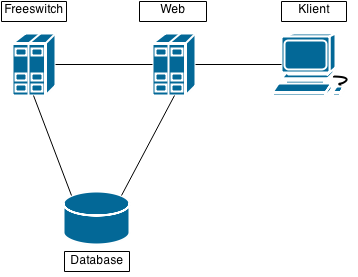
\includegraphics[scale=0.8]{images/systemdiagram.png}
\caption{Diagram over projektets komponenter}
\label{fig:systemdiagram}
\end{figure}

\section{Database}
Datamodellen er lavet så først har man organisationer, som fortæller hvilken virksomhed der skal sendes regninger ud til og hvordan de ønsker dem, samt at den samler flere receptioner. En reception er den kontekst som der bliver ringet ind til. Så i større virksomheder vil der være flere som f.eks. afdelinger eller forskellige butikker rundt omkring i landet og i små virksomheder vil der typisk kun være én reception. En reception består af information om blandt andet hvordan de ønsker håndtering af sælgere, hvad deres CVR numre er og helt lavpraktisk hvad addressen er eller hvad deres åbningstider er og ikke mindst dens kaldplan. 
\begin{figure}[ht!]
\centering
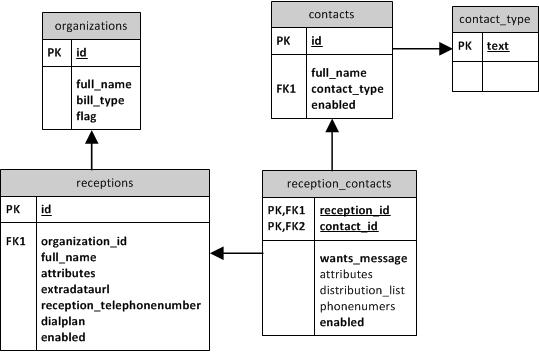
\includegraphics[scale=0.7]{images/ER_Basic.png}
\caption{Udsnit af database skemaet. PK er Primary key. FK er Foreign Key. Tekst i fed skrift er obligatoriske felter.}
\label{fig:erbasic}
\end{figure}

En virksomhed er ikke noget uden deres medarbejder, så til dem er der kontakter som beskriver personen ved deres navn. Det er først i forbindelse med en reception at en kontaktperson har det meste af sin information, som hvad deres telefonnumre og email er, samt information omkring hvad de har af ansvar og hvem deres backup personer er, og den information gemmes i ReceptionContacts tabllen.
Databasen har en flere tabeller end beskrevet her og diagrammet for det fulde database skema kan findes i bilaget.

\section{Server}
Serveren er modelleret op efter MVC arkitekturen, da det passer godt til hvordan en websevrer kan sættes sammen og er godt til at holde de forskellige dele adskildt. Derved har den en række controllere som står for at håndtere forespørgelserne, samt nogle modeller så når dataen kommer ned fra databasen eller fra klienterne, så har man nogle typestærke objekter man kender strukturen af. Serveren har også nogle views der tager sig af at præsenteres modellen i et format der sendes til klienten. 
Serveren er bygget op efter REST principperne, som der kommes mere ind på senere i kapitlet. 

\pagebreak
\section{Brugerfladen}
Brugerfladen er blevet skitseret i samarbejde med AdaHeads K/S og Responsum K/S.
Den er bygget op, så i venstre side har man en menu hvor man kan vælge imellem organisation-, reception-, kontakterperson- og kaldplans-vinduet. Alle 4 vinduer er bygget op omkring 3 søjler for at holde det ensartet.

\subsection{Organisationer}
\begin{figure}[ht!]
\centering
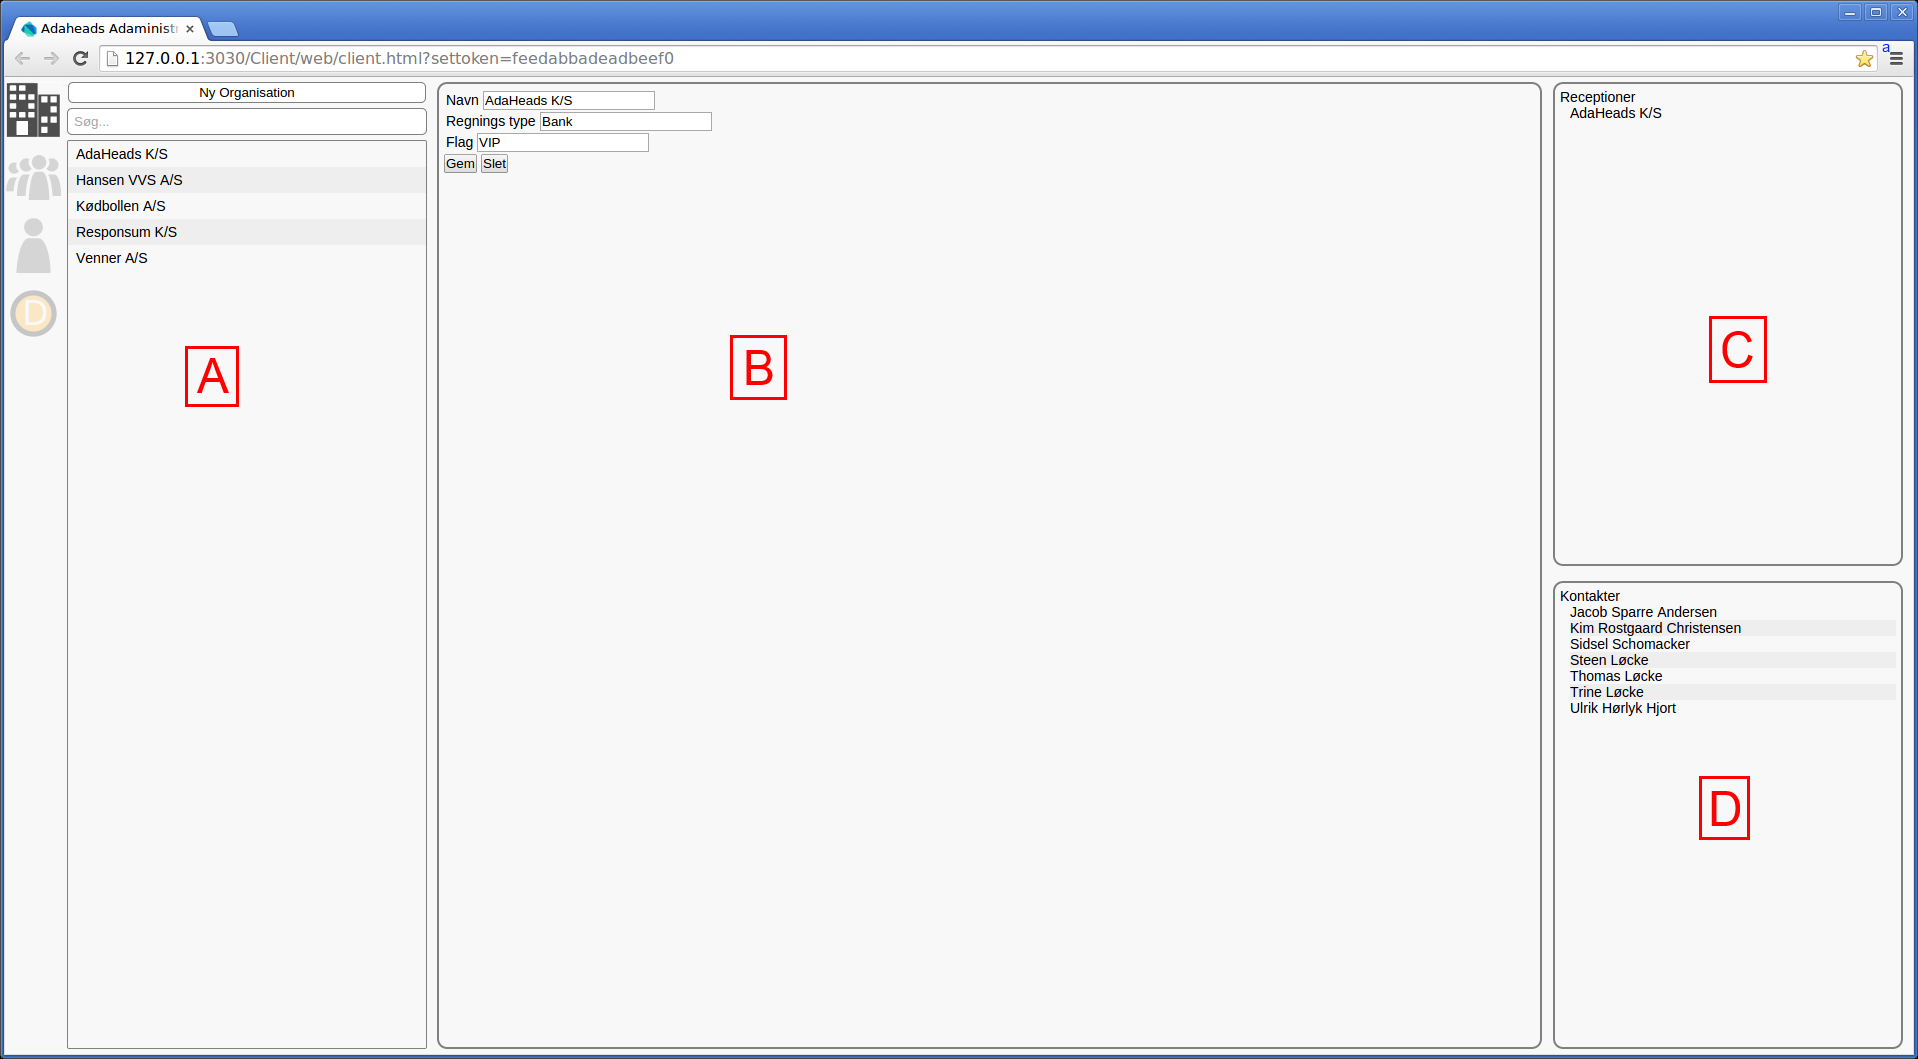
\includegraphics[width=\textwidth]{images/screen_org.png}
\caption{Organisation redigering}
\label{fig:screenorg}
\end{figure}
\begin{enumerate}
	\item[A.] {Set fra toppen mod bunden er der først en knap hvor der kan oprettes nye organisationer, efterfulgt af et søgefelt hvor man kan filtrere på listen af alle organisationer i systemet}
	\item[B.] {Informationen omkring den valgte organisation, samt mulighed for at gemme ændringer og slette organisationen}
	\item[C.] {Liste over receptioner tilknyttet den givende organisation}
	\item[D.] {Liste over samtlige kontakter der er tilknyttet organisationen}
\end{enumerate}

%På organisations vinduet kan man ude i venstre side se en liste af alle organisationer som er tastet ind, og i toppen af den kan man enten skrive i søgefelter som filetere listen %neden under eller trykke for at oprette en ny. 

%I midten kan man indtaste information omkring den pågældende organisation. I den højre søjle er der to lister. Den ene med receptioner og den anden med kontaktpersoner der tilhører den valgte organisation.

\pagebreak
\subsection{Receptioner}
\begin{figure}[ht!]
\centering
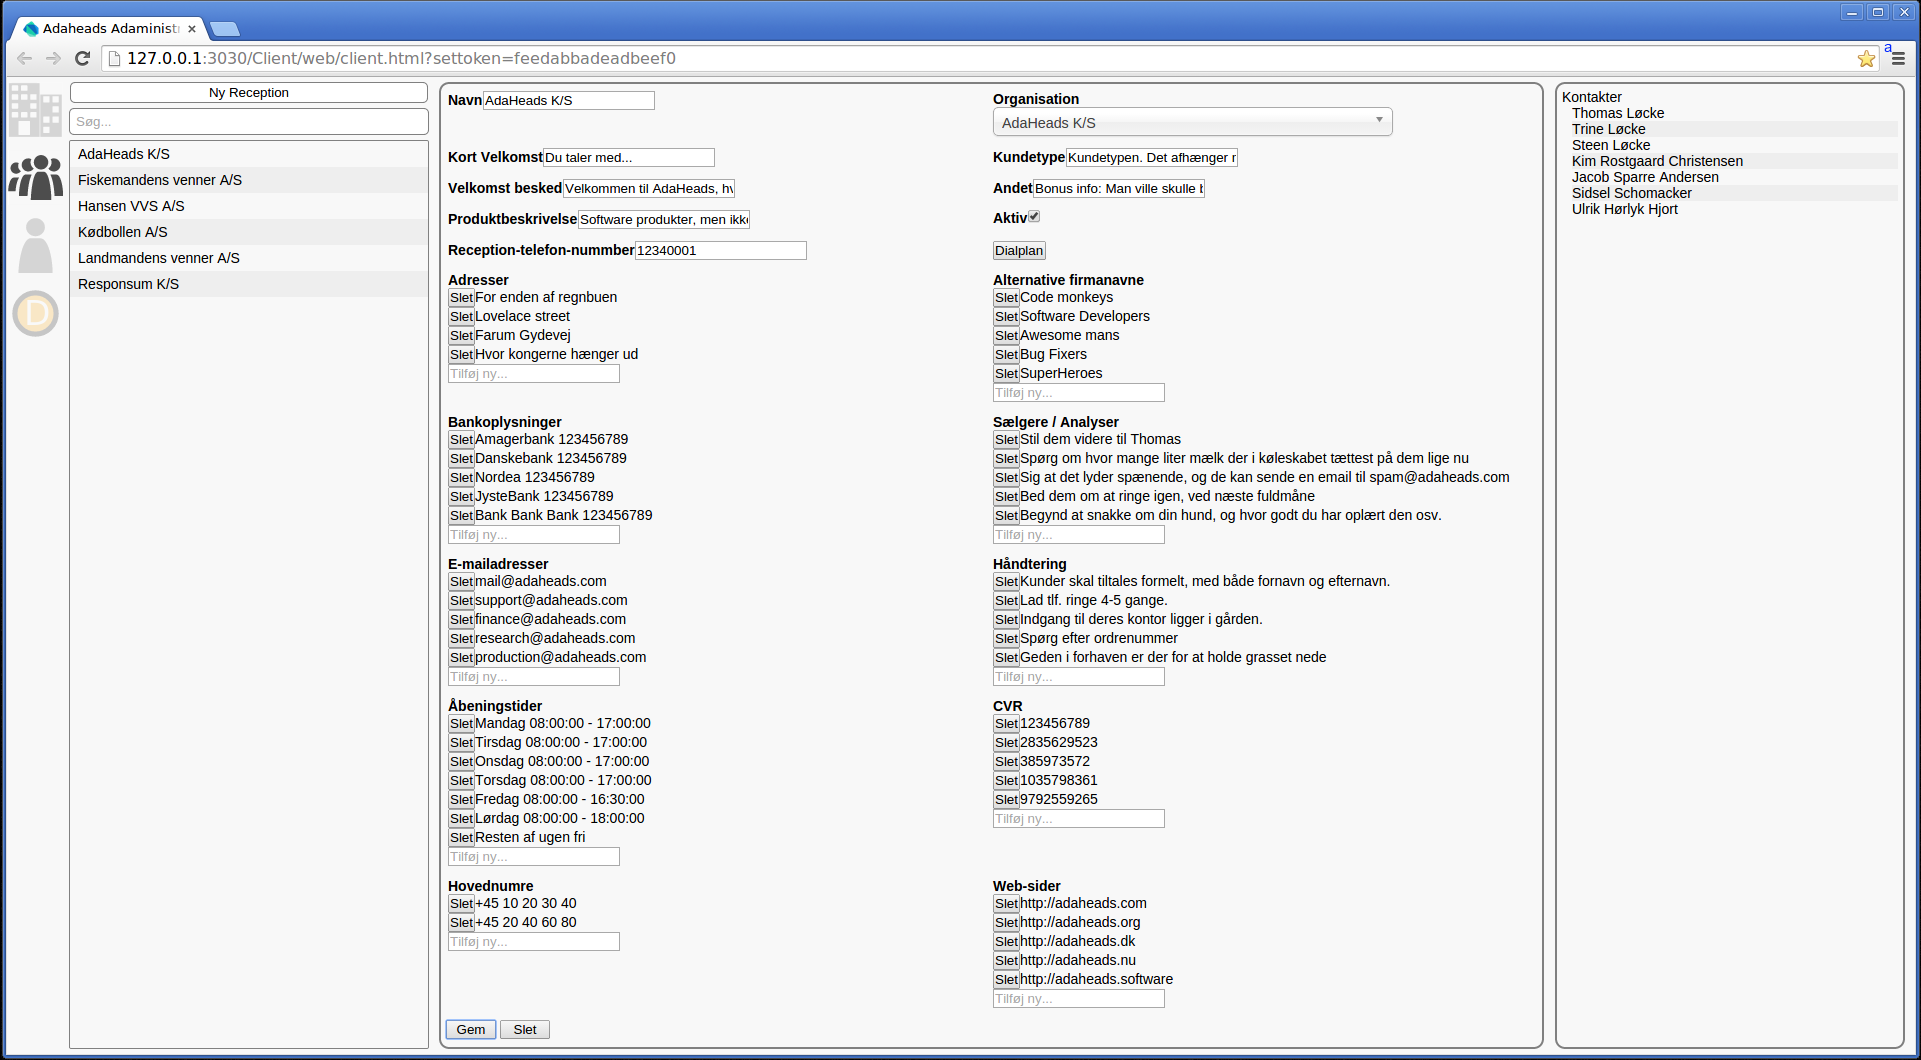
\includegraphics[width=\textwidth]{images/screen_rec.png}
\caption{Reception redigering}
\label{fig:screenrec}
\end{figure}
\begin{enumerate}
	\item[A.] {Set fra toppen mod bunden er der først en knap hvor der kan oprettes nye receptioner, efterfulgt af et søgefelt hvor man kan filtrere på listen af alle receptioner i systemet}
	\item[B.] {Informationen omkring den valgte reception, samt mulighed for at gemme ændringer og slette organisationen. Receptionen indeholder mange lister hvor man kan ved at trække i rækkerne ændre på deres rækkefølge og ved et tryk har man mulighed for at ændre i teksten. I bunden af alle listerne er der et felt hvor der står "Tilføj ny...". Hvis man skriver en tekst i den og afslutter med enter, vil der blive oprette en ny række med den skrevende tekst i}
	\item[C.] {Liste over kontakter tilknyttet den givende reception der ved et tryk på en kontakt kan sende brugeren hen til siden hvor kontakten kan redigeres}
\end{enumerate}

%Reception vinduet er lavet i meget samme stil som organisationvinduet med de 3 søjler. Det har også, hvis vi starter fra toppen i venstre siden, en søjle med en knap hvor der oprettes nye receptioner, et søgefelt for listen neden for, der indeholder alle receptioner. 

%I midten er søjlen med informationen omkring en reception samt to knapper der giver muligheden for enten at gemme de ændringer der er indtastet eller at slette den valgte reception. 

%Til højre er der en søjle med alle kontaktpersoner der har en forbindelse til den valgte receptionen.

\pagebreak
\subsection{Kontaktpersoner}
\begin{figure}[ht!]
\centering
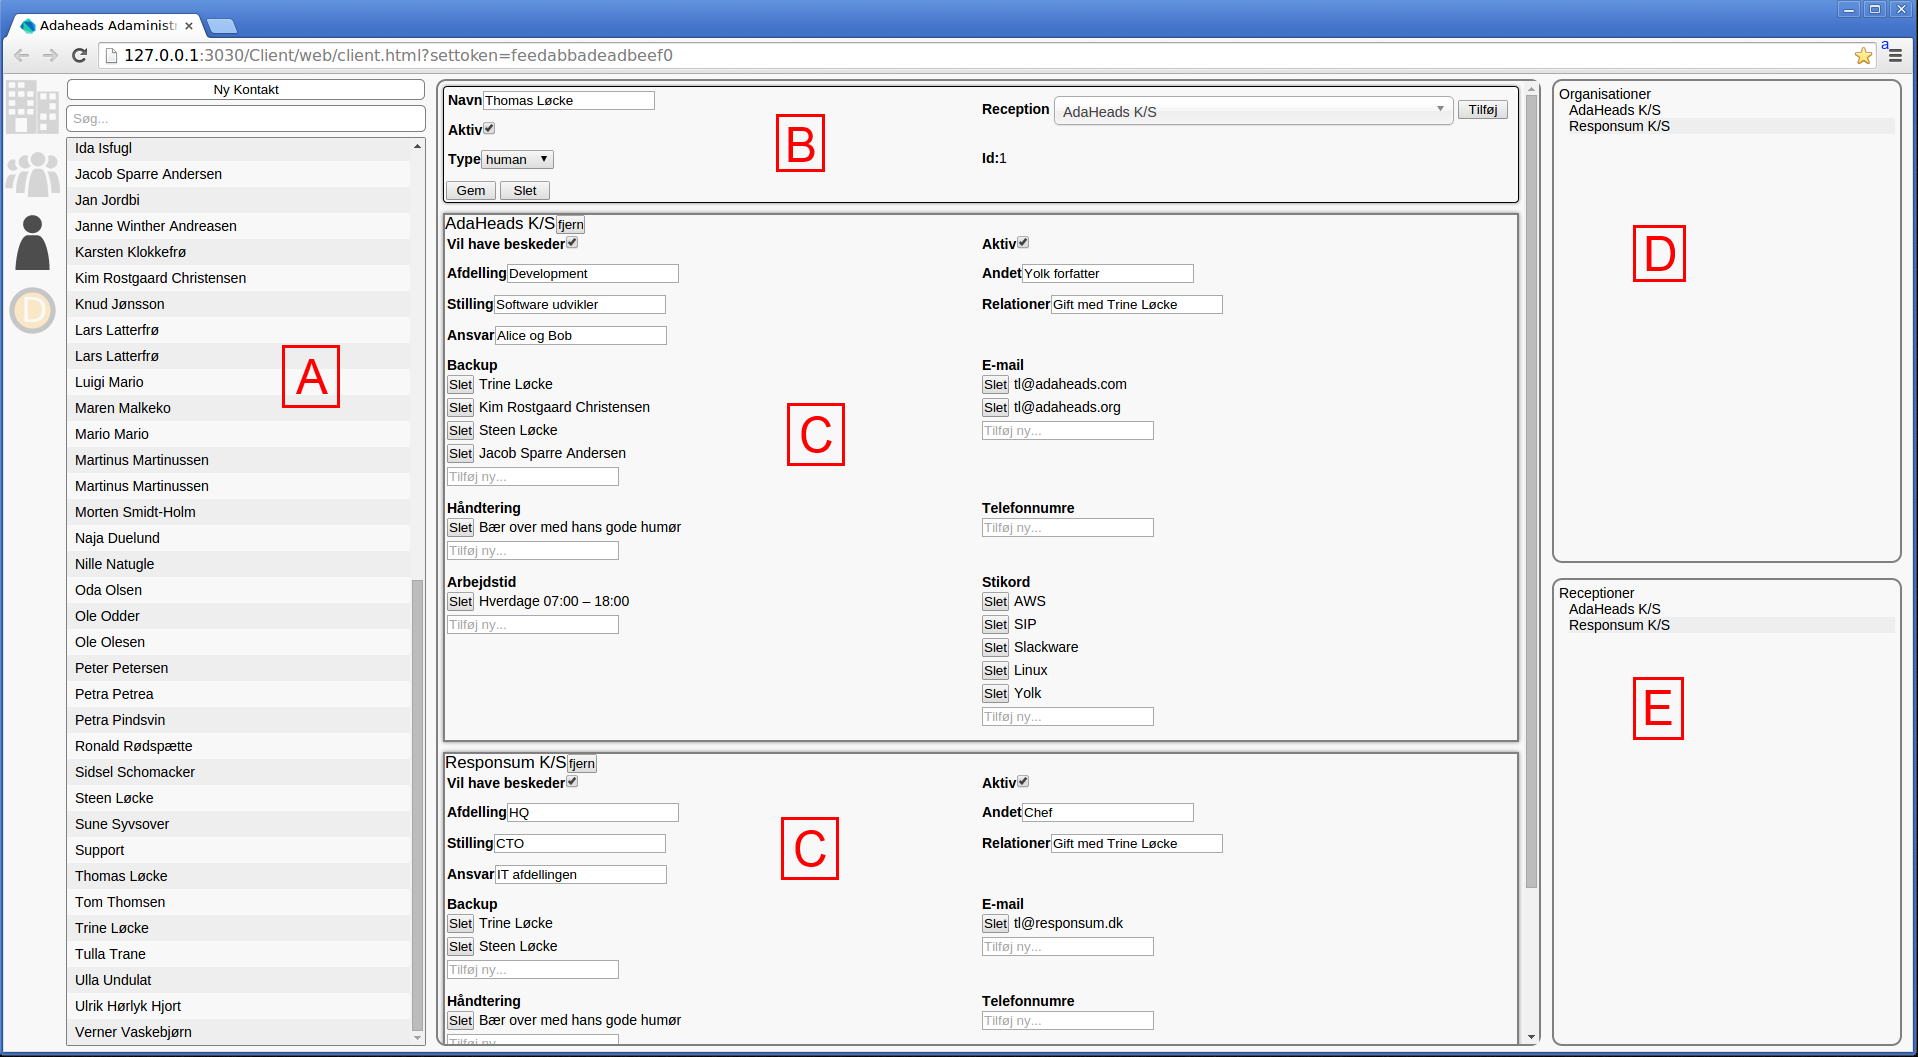
\includegraphics[width=\textwidth]{images/screen_con.png}
\caption{Kontakter redigering}
\label{fig:screencon}
\end{figure}
\begin{enumerate}
	\item[A.] {Set fra toppen mod bunden er der først en knap hvor der kan oprettes nye kontaktpersoner, efterfulgt af et søgefelt hvor man kan filtrere på listen af alle kontakter i systemet}
	\item[B.] {Staminformationen for den valgte kontakt person, samt mulighed for at gemme alle ændringer til kontakt, slette kontakten eller tilføje kontakten til en reception}
	\item[C.] {For hver reception en kontakt er med i, kommer der en boks med den tilknyttede information i}
	\item[D.] {Liste over samtlige organisationer som kontaktpersonen har en tilknytning til}
	\item[E.] {Liste over samtlige receptioner som kontaktpersonen har en tilknytning til}
\end{enumerate}
%I vinduet for kontaktpersoner er der lige som i de forrige to, opret knap, søgefelt og i vinduet her er det en så en liste over kontaktpersoner. I toppen af søjlen i midten er der information omkring en kontaktperson, hvor der er mulighed for at tilknytte en kontakt til en reception. Har en kontaktperson en tilknytning til en reception, så optræder der en boks for hver reception med alt information tilknyttet til den relation. I højre side er der to lister henholdvis hvilke organisationer og receptioner som kontakten optræder i.

\pagebreak
\subsection{Kaldplan}
\begin{figure}[ht!]
\centering
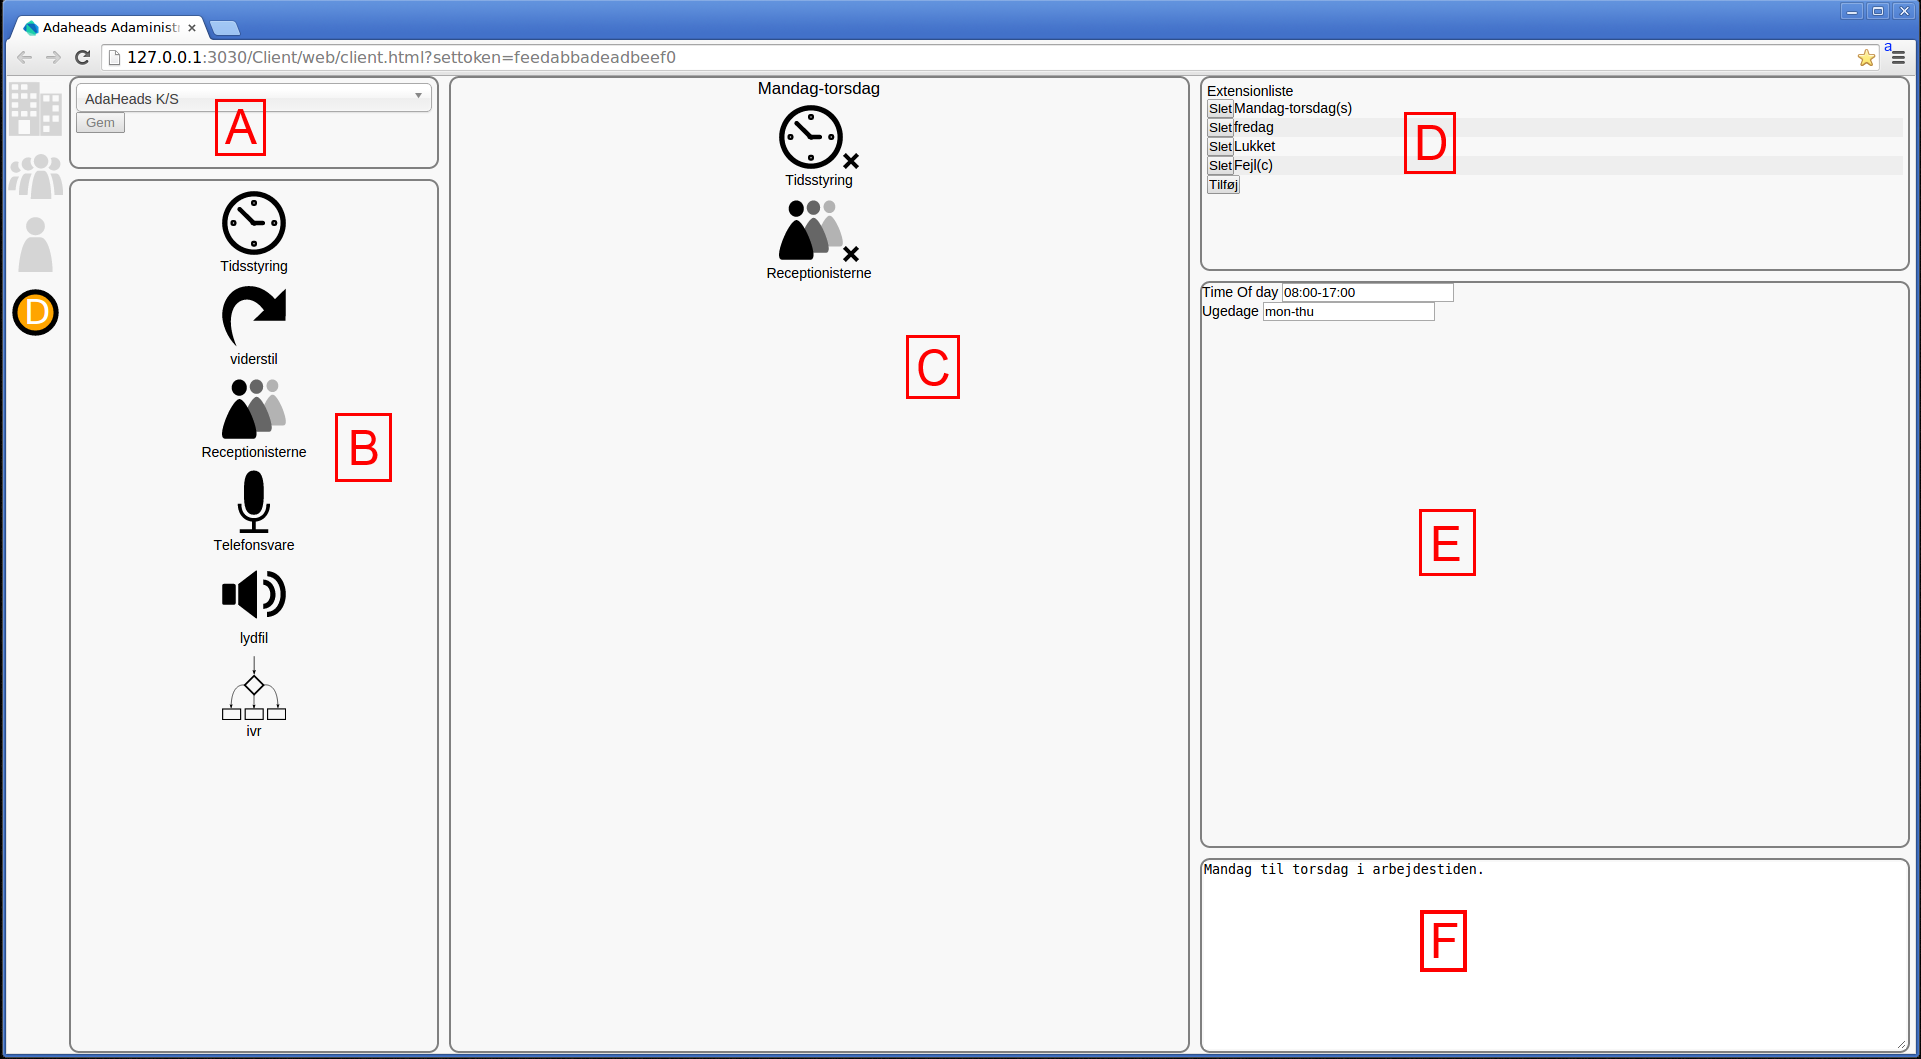
\includegraphics[width=\textwidth]{images/screen_dialplan.png}
\caption{Redigering af kaldplaner}
\label{fig:screendialplan}
\end{figure}
\begin{enumerate}
	\item[A.] {En knap til at gemme ændringer samt en boks som hvis man trykke på den folder den ud til en liste af receptioner med et søgefelt så man kan vælge hvilken receptions kaldplan der skal ændres.}
	\item[B.] {En liste med den betingelser og handlinger man kan sætte ind i en kaldplan}
	\item[C.] {Visning af den valgte extension's betingelser og handlinger}
	\item[D.] {Liste over de extensions der er oprette i kaldplanen}
	\item[E.] {Viser indstillingerne for den valgte kaldplanskomponent, eller extension}
	\item[F.] {Felt til at skrive en kommentar til den valgte komponent, som der kræves fra krav F08}
\end{enumerate}

\pagebreak
\section{Kaldplan compiler}
Freeswitch er bygget op af en kerne der i sig selv ikke kan bruges som PBX, men med de moduler som følger med kan den bruges til at forbinde IP telefoner eller andre PBX'er, transkode lyd, afspille IVR menuer altså hvad man kræver af de traditionelle PBX og hvis det ikke er nok kan man altid skrive sit eget modul.

Når der kommer et opkald ind i telefonanlægget, skal Freeswitch vide hvordan det skal håndtere opkaldet.
I Freeswitch kan man skrive sin kaldplan i en række af programmeringssprog, men som standart bliver der brugt et modul kaldet mod\_dialplan\_xml og som navnet fortæller så bruger den XML til at beskriver kaldplanen. Der er også den mulighed at lave det, de kalder en outbound socket som fungere ved at man forbinder til deres socket, og der hvor den før hen havde gået ned og læst hvilke applicationer der skulle afvikles, så spørger Freeswitch istedet for på denne forbindelse. 

Adaheads K/S valgte at bruge mod\_dialplan\_xml og derved skrive deres kaldplan i XML. Det giver den fordel at mod\_dialplan\_xml er et gennemprøvet modul og når der skal laves ændringer til en kaldplan så kan man ændre i filerne og bede Freeswitch om at genindlæs dens kaldplaner, hvilket ikke giver nogen nede tid og så er det også en mere stabil løsning. Den mere dynamiske tilgang med en socket er mere fleksibelt, men den statisk udgave ser ud til at kunne det Adaheads kræver af det.

AdaHeads K/S valgte at bruge mod\_dialplan\_xml og dermed skrive deres kaldplaner i XML. Det giver dem en række fordele i forhold til at bruge Freeswitch's outbound socket. 
Først og fremmest skal der ikke udvikles og vedligeholdes noget nyt program til at kommunikere over deres outbound socket. 
Det næste er at når en dialplan skal ændres kan man blot ændre i XML filerne og bede Freeswitch om at genindlæse dem, hvor derimod at hvis man havde et program skulle man sætte redundante instanser ind, så man kan tillade sig at tage det ned for at starte den updateret udgave. 
For det tredje så de kriterier som et opkald dirigeres efter vides mange dage på forhånd, så de dynamiske muligheder fra en socket har ikke vist sig nødvendige endnu.

\pagebreak
\section{Mod\_Dialplan\_XML}
\label{sec:moddialplanxml}
En kaldplan er bygget op af en række lag, som det kan ses på figur~\ref{fig:xmldialplan}. 
\begin{figure}[ht!]
\centering
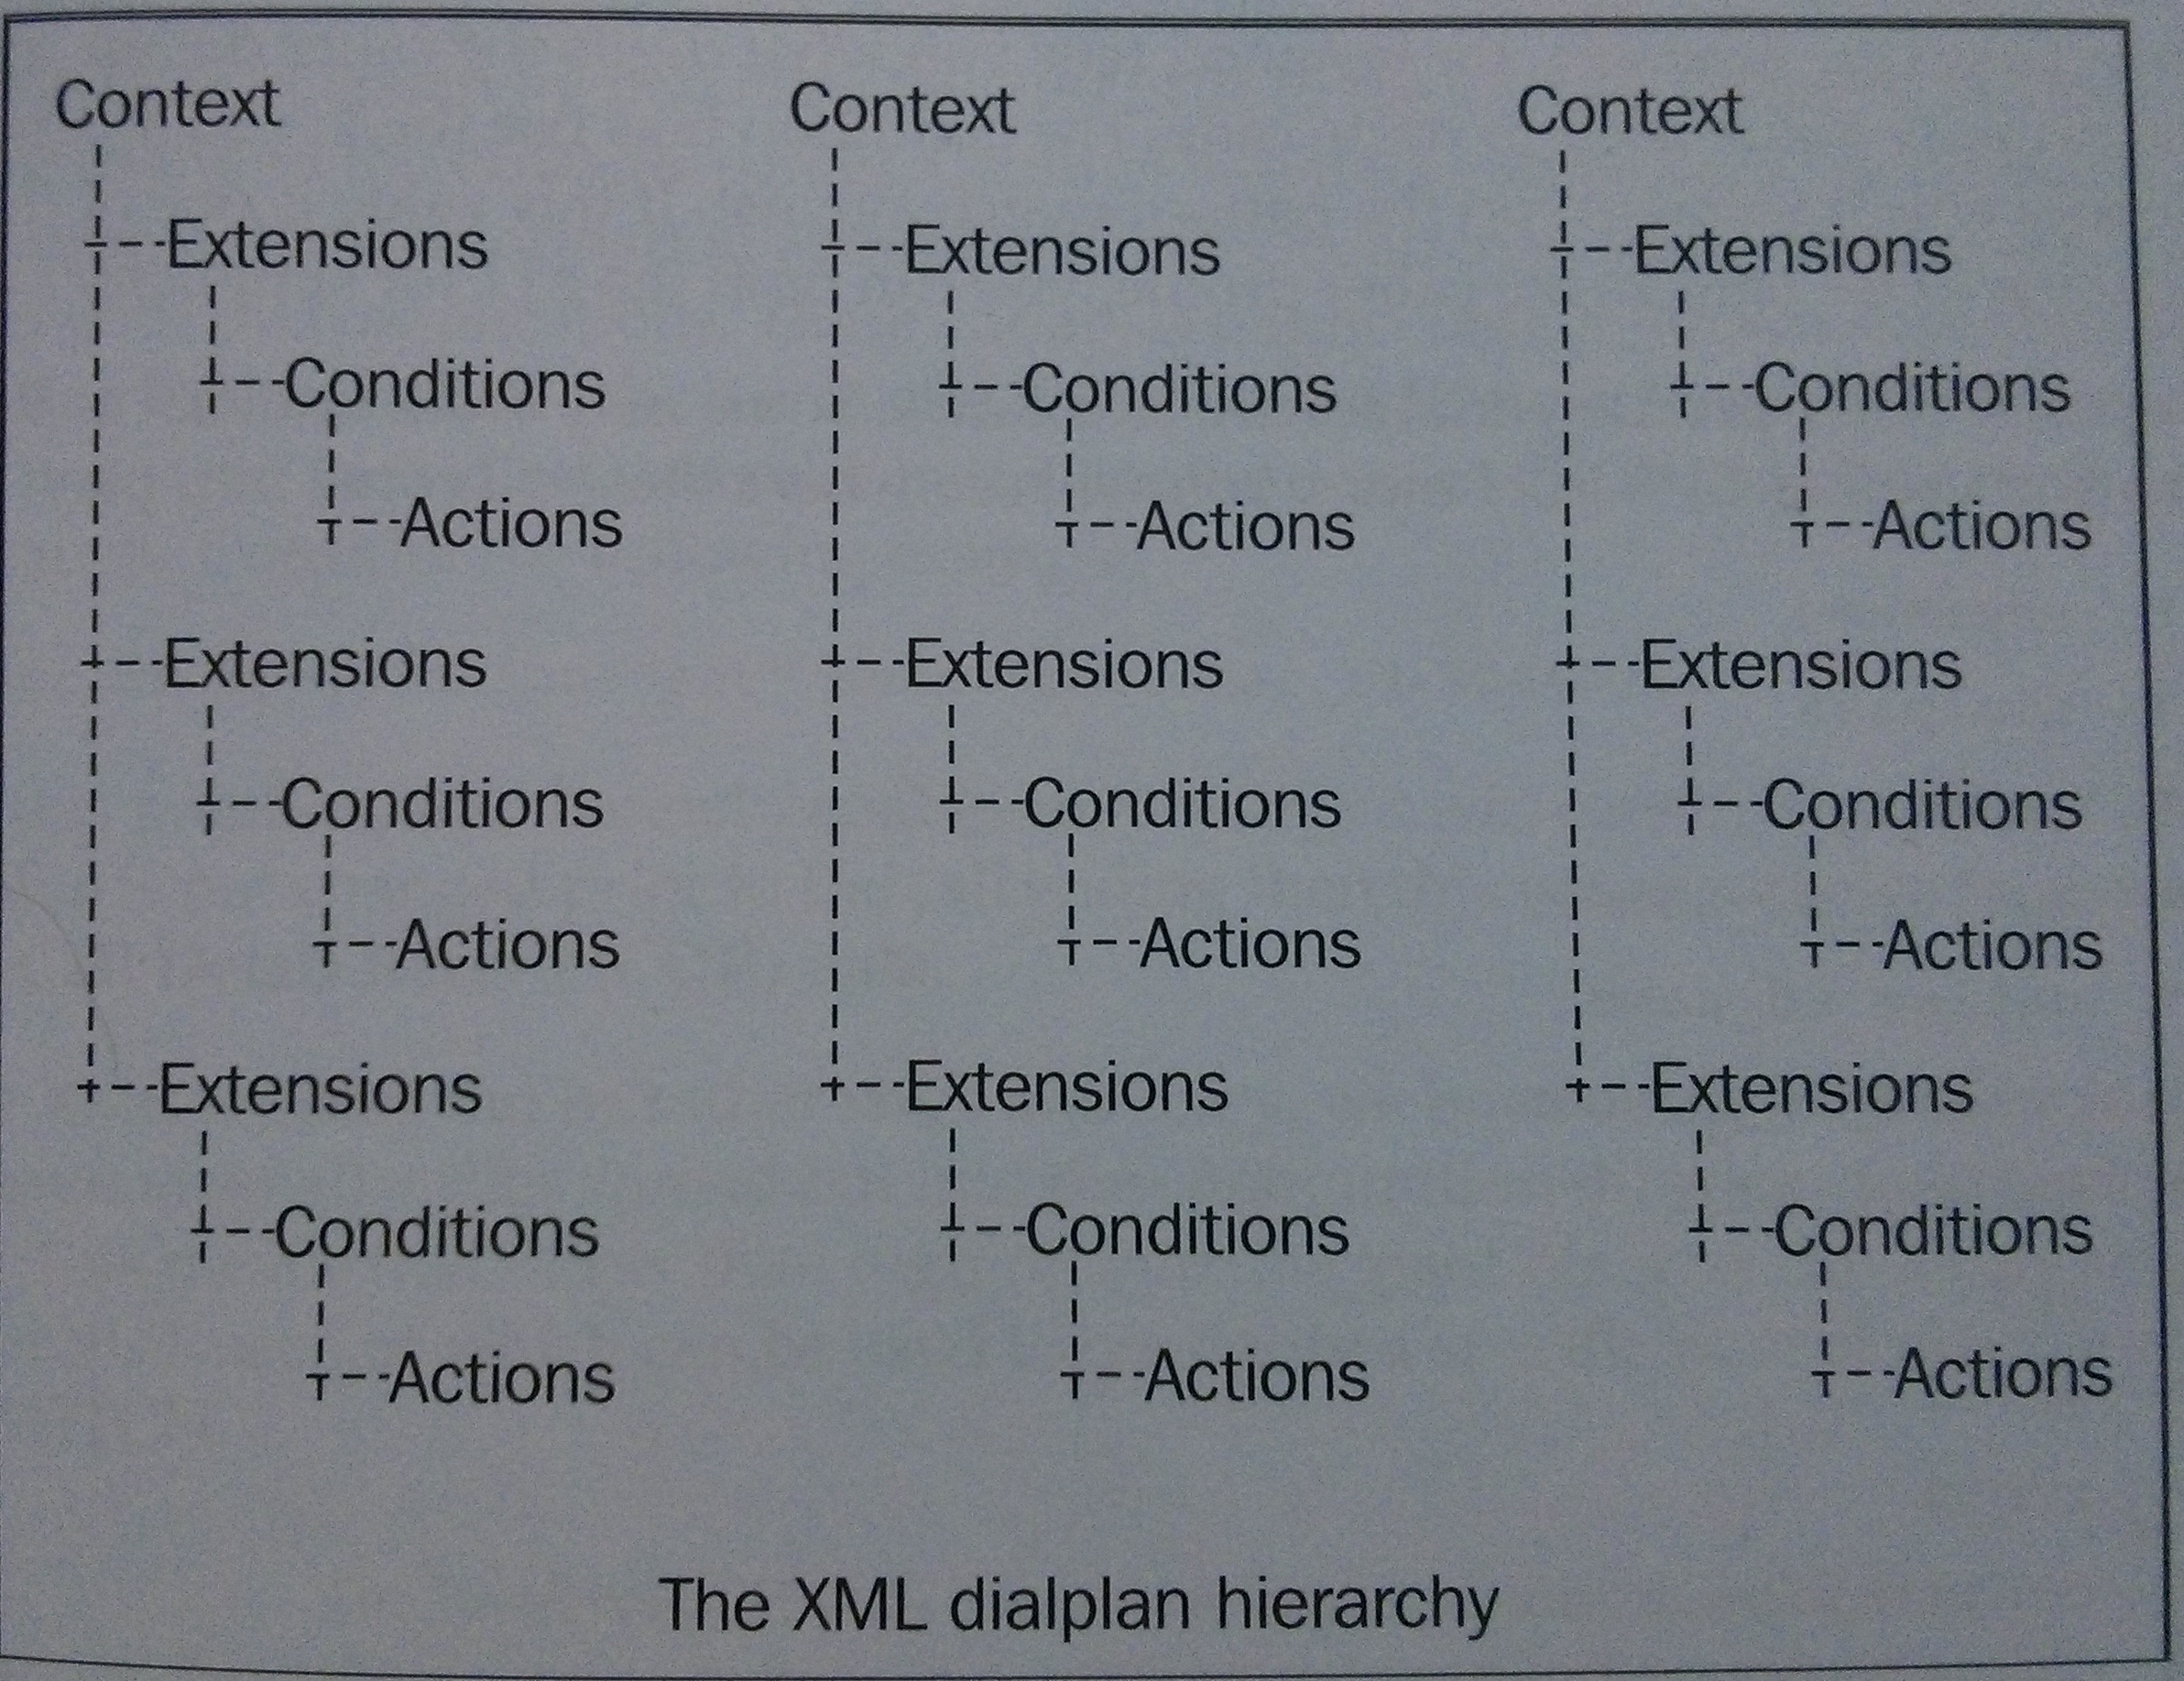
\includegraphics[scale=0.12]{images/dialplanstructure.jpg}
\caption{Strukturen for en XML kaldplan\citep{freeswitch12}}
\label{fig:xmldialplan}
\end{figure}

%\linebreak 
Det først lag er Context. 
En Context er specificeret ved et unikt navn, den kan bestå af flere extensions og en kaldplan kan have flere contexts. Når man registrer en telefon, eller en PBX så konfigureres en context der ringes i. Det har den fordel at man kontrollere hvilke extension som kan ringes ind til fra hver telefonerne og for hver af PBX.

Det næste lag er for extensions. En extension er en gruppering af conditions.
Conditions er som navnet beskriver, de betingelser der skal opfyldes. 
Hvis en condition evaluere til sandt udføres dens actions og hvis ikke så udføres dens anti-actions.
En condition har indbygget funktionalitet til at tjekke på en masse ting omkring tid. F.eks. om det er en bestemt ugedag, eller om klokken er mellem et specificeret interval, hvilket år det er osv. Men udover det kan man kalde andre applikationer og ved hjælp af Regular Expression der bruges til at tjekke svaret, udbygge det til at tjekke hvad som helst. 

Actions og anti-actions er det samme, det eneste der skiller dem ad, er i hvilke omstændighed de bliver udført. Actions er bygget op helt simplet, ved at man specificere et applikationsnavn og dens parameter. For eksempel hvis man ønsker at afspille en lydfil, så sætter man applicationsnavnet til \enquote{playback} og parameteren til stien til filen, så det kunne komme til at se således ud: \linebreak <action application="playback'' data="/home/thomas/welcome.wav"/>

\section{REST}
\label{sec:rest}
Serveren er designet, som nævnt tidligere, i følge principperne bag REST. \linebreak
REST (\textbf{RE}presentational \textbf{S}tate \textbf{T}ransfer) er en web arkitektur der blev opfundet af Roy Fielding i hans ph.d.-afhandling. I den beskriver han at denne arkitektur bygger oven på HTTP og at serveren som klienten snakker med skal være tilstandsløs. Det har en række fordele. Når transportlaget ikke skal holde nogen tilstand, så kan det spare på de fysiske ressourcer og på den måde opnå højere skalerbarhed. Det betyder også at man kan sende forspørgelser parallelt og at der kan køre flere instanser af serveren, og klienten behøver ikke vide hvilken en der snakkes med.
REST er bygget op efter tanken at man arbejder med resourcer, som der kan hentes, oprettes, ændres og slettes igen baseret på et mønster der tager brug af \enquote{method} feltet i HTTP.

Hvis man f.eks. skulle tage udgangspunkt i receptionerne, så kan man hente en bestemt reception på addressen /reception/<id> hvor <id> referere til et tal eller en tekst der kan identificere en bestemt reception og ved bruge method GET, fortæller man at den skal hentes. Spørges der ind til den samme addressen med method valgt til DELETE, så vil den slette receptionen. Lige ledes kan man bruge PUT til at updatere og POST til at oprette nye.

\chapter{Implementering}

I dette kapitel vil der blive gennemgået forskellige dele af systemet.

\section{Kaldplan compiler}

Til at bygge en kaldplan er der lavet et bibliotek kaldet libdialplan der er skrevet i Dart. libdialplan er modellen for de kaldplaner som brugeren laver ude i klienten, i en struktur der efterligner hvad brugeren ser, for nemt at kunne genindlæse en kaldplan. Derfor har hvert komponent sin egen klasse i biblioteket, med en række felter svarende til de indstillinger som brugeren har for komponenten. Dette bibliotek genbruges i compileren, for dermed nemt at kunne indlæse den givende kaldplan i typestærke elementer.


Når en kaldplan er blevet bygget i klienten og gemt i databasen skal den oversættes til det format som Freeswitch forstår -- og til det bruges compileren. Når et opkald kommer ind i PBX'en går det ind i en context kaldet \enquote{public}, derfra skal opkaldet så sendes ud til den rette reception. Derfor er det første som compileren laver, at oprette en extension i \enquote{public} contextén hvorfra opkaldet bliver sendt ud til den pågældenes receptions context.
Ved at lave en context for hver reception, så giver det muligheden for at hvis der ikke er en extension der har alle sine conditions opfyldt og der ikke at lavet nogen anti-actions til at tage højde for det eller at der på andenvis er opstået en fejl i forbindelse med conditions, så kan man fordi den leder fra top til bund, placere i bunden en extension hvor dens condition altid er opfyldt \citep{minessale2012freeswitch}. Så hvis der for eksempel ikke er taget højde for et tidsinternal, så falder opkaldet til sidst altid ned i den. Det betyder også at der kun kan være en per context.

\section{Server}

Når en forespørgelse kommer ind til webserveren skal den først finde ud af hvilken resource som der spørges efter. Til det er biblioteket Route\footnote{Biblioteket kan hentes her http://pub.dartlang.org/packages/route} brugt som benytter sig af regulære udtryk til at viderstille forespørgelse til den rette funktion.
Route har mulighed for at man lave nogle filtre der tjekkes igennem først. Det er blevet udnyttet til at tjekke for om forespørgelse har en token og om den er gyldig til at verificere at de er logget ind. Hvis det er tilfældet så sendes forespørgelsen ud til den rette controller. 

Spørges der f.eks. efter at få oprette en ny reception, samler controllerne informationen sammen fra forespørgelsen og sender det til databasen der svare med id'et på den nye reception hvis det gik godt. Det id bliver så sendt tilbage til klienten igen.

\begin{figure}[ht!]
\centering
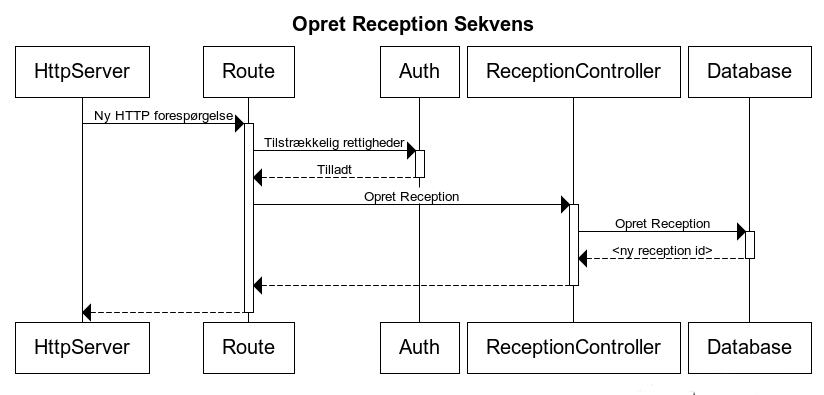
\includegraphics[width=\textwidth]{images/serversequence.png}
\caption{Når man kalder serveren for at oprette en ny reception}
\label{fig:serversequence}
\end{figure}

\pagebreak
\section{Migrering}
Når Responsum K/S skal lave skiftet til det nye system er det vigtigt at kunne få deres data med over. Til det er der blevet skrevet et lille program i Dart. Programmet er skrevet i Dart fordi modellen og forespørgelserne til databasen allerede var lavet i Dart, hvilket gjorder det hurtigt at låne der fra. Det gamle systems database var en Microsoft Access database og fordi at Dart ikke har support for at læse Access databaser blev der brugt et andet program \enquote{mdb-export} der gemmer tabellerne som kommasepareret filer. Migreringsprogrammet indlæser filerne til typestærke objekter og flytter det til felter i det nye databaseskema for så at gemme det i databasen.
\chapter{Test}
Man kan teste sine programmer på mange forskellige måde, man kan blandt andet lave unit test, integration test og acceptance test. Unit test er test af mindre dele af programmet. Meningen med dem er at de er små og hurtige, så når der arbejdes på en lille krog af programmet, så har man flere test til det, som man kører igen og igen for at sikre sig at når man udvikler det at man ikke ødelægger noget på vejen.
Integretions test er hvor der tests om hvor vidt at et program overholder deres interface. Så her ser man ikke på de små komponenter et program består af men om det overordnet virker som det skal.
Acceptance test er når produktet afleveres til kunden og der undersøges om det lever op til deres krav.

I dette projekt er blevet lavet automatiske integrations test til serveren. Testene blev skrevet i Python, da det har nogle gode test biblioteker og fordi så kunne det nemt intregreres med Adaheads nuværende test miljø som netop også kører Python.
For at tests om der nu leveres data tilbage i det rette format, så bruges der JSON\_Schema til at validere op i mod. JSON\_Schema er skrevet JSON og tjekker om visse nøgler er tilstede, eller om værdierne overholder et regex udtryk eller hvis det er et tal kan man validere at værdien ligger imellem et interval.

\chapter{Konklusion}
På de 12 uger som projektet løb over er der kommet en række af programmer ud. Det starter med migraring af stamdata over til det nye system, efterfuldt af webserver og webside kombination til serviceagenterne og til sidste rundet af med en compiler til at lave dialplans. 
Projektet i samarbejde med Adaheads K/S og Responsum K/S har sat godt igang i processen om at få udviklet deres administrative del af deres system men det er bestemt ikke færdig endnu.
%\include{Chapter2}                                 %Chapter 2



%\appendix
\begin{appendices}
\chapter{Database diagram}
I tillæg til det tidligere beskrevede 
Det fulde database diagram har ud over det tidligere beskrevede omkring organisationer, receptioner og kontakter også nogle tabeller for at håndtere brugerrettigheder, beskeder der muligvis skal sendes ud til en eller flere medarbejdere, kalender begivenheder og opsamling af opkalds information.

%Beskriv noget om navngivningen
%Postgres har understøttelse for JSON, Validering og Query. 
%JSON giver mulighed for fleksibel udvikling
%Marker tabeller brugt i dette projekt op.

Se næste side.

\pagebreak
\begin{figure}[ht!]
\centering
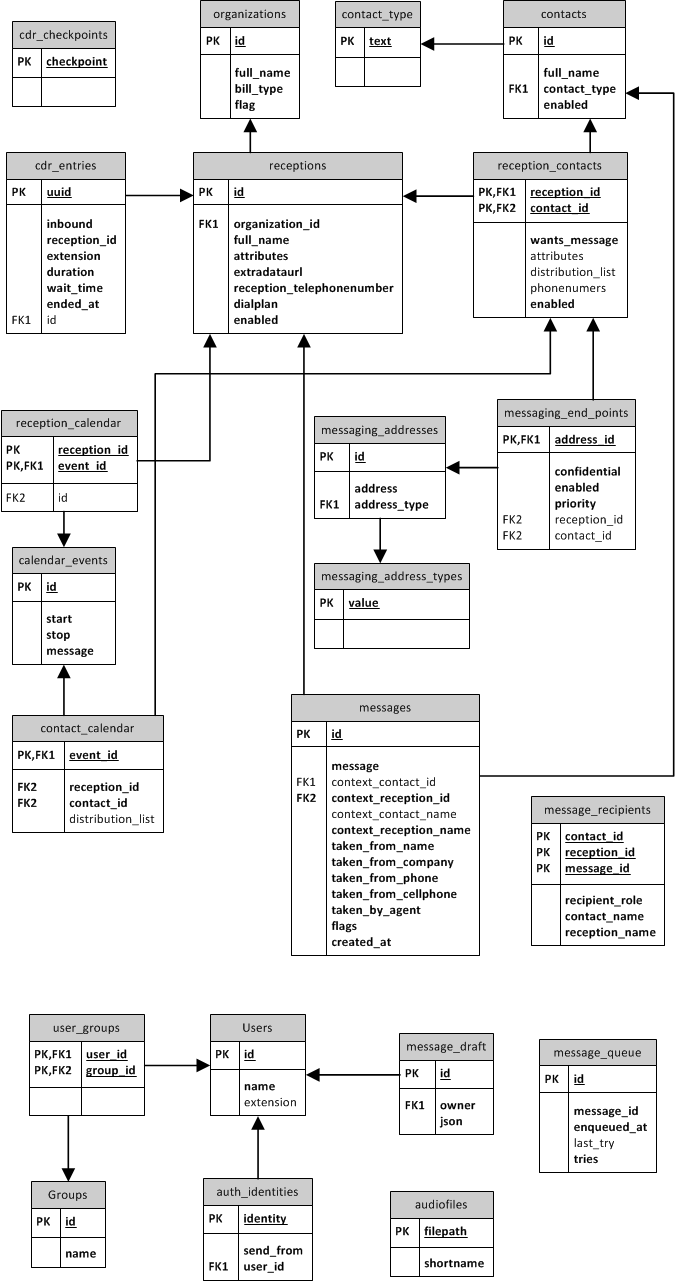
\includegraphics[height=\textheight]{images/ER_Full.png}
\caption{Det fulde database skema}
\label{fig:erfull}
\end{figure}
                                 %Appendix A
\end{appendices}

%-----------
% Backmatter
%-----------
\backmatter


\chapter*{Terminologi}

%\paragraph{GPL}

\begin{description}
	\item[Dart] er et sprog fra Google til at afløse Javascript, der udkom i version 1.0 i november 2013. Dart er lavet til at køre hurtigere end Javascript ved blandt andet at indføre klasser, da det betyder at et object ikke kan ændre signatur når først programmet køre\citep{walrath2012dart}.
	
	\item[Extension] er en gruppering af betingelser og handling i en kaldplan. Se kapitel~\ref{sec:moddialplanxml}
	
	\item[Freeswitch] er en soft-PBX, altså en PBX skrevet i software.
	
	\item[Kaldplan] er den opskrift der fortæller hvordan et opkald skal dirigeres i en PBX og videre.
	
	\item[GPL] er en lisence der sikre at brugeren er fri til at bruge, læse, kopiere og ændre programmet.	
	
	\item[MVC] (Model View Controller) er en arkitektur der først har modellen, altså typer til at opbevare data så det giver mening i forhold til domænet. Der efter er der view som via det data der kommer fra modellen, at lave en repræsentation af dataen som sendes ud. TIl sidste Controller der forbinder det hele, og som har alt bussiness logikken.
	
	\item[PBX] (\textbf{P}rivate \textbf{B}ranch E\textbf{x}change) er et alment udbredt udtryk for lokale telefonanlæg. Altså det system der tager sig af at håndter opkald.
	
	\item[Receptionist] er en medarbejder som tager opkald og sørger for at omstille eller tage imod en besked fra opkalder.
	
	\item[REST] er en tilstandsløs arkitektur der opererer over HTTP. Se kapitel~\ref{sec:rest}
	
	\item[Regular Expression] eller på dansk kendt som Regulære Udtryk. Er et sprog der kan sammenligne tekster og finde matches eller erstatte dele af teksten.
	
	\item[Serviceagent] er en der sørger for at holde data omkring firmaerne opdateret, så receptionisterne har den rigtige information.
\end{description} 

\chaptermark{Bibliography}
\renewcommand{\sectionmark}[1]{\markright{#1}}
\sectionmark{Bibliography}
\addcontentsline{toc}{chapter}{\bibname}        %Force addition of Bibliography to TOC
\bibliographystyle{plain}                           %Use alpha codes for references
\bibliography{References}                           %Bibliography file called
\end{document}
% % % EOF % % %